
\documentclass{article}%%%%article template
\usepackage{lineno}
\usepackage{amsmath}
\usepackage{graphicx}
\usepackage{cite}
%\usepackage{changes}
%\usepackage[sorting = none, backend = bibtex, style=numeric-comp]{biblatex}
%\addbibresource{Accretion_erosion.bib}
% begin document
\begin{document}

%%%% Article title to be placed here
Insert the article title here


%X. X. Nyssa Silbiger$^{1}$, X. Second author$^{2}$ and X. Third author$^{3}$}

%%%%%%%%% Insert author address here
%$^{1}$University of California, Irvine\\
%$^{2}$Second author address\\
%$^{3}$Third author address

%%%% Subject entries to be placed here %%%%
xxxxx, xxxxx, xxxx

%%%% Keyword entries to be placed here %%%%
xxxx, xxxx, xxxx

%%%% Insert corresponding author and its email address}

%%%% Abstract text to be placed here %%%%%%%%%%%%
\linenumbers %% add line numbers
\section{abstract}
The abstract text goes here. The abstract text goes here. The abstract text goes here. The abstract text goes here.
The abstract text goes here. The abstract text goes here. The abstract text goes here. The abstract text goes here.

%%%%%%%%%%%%%%%%%%%%%%%%%%%

%%%%%%%%%% Insert the texts which can accommodate on firstpage in the tag "fmtext" %%%%%


\section{Introduction  }
%%%% Insert A head here

Coral reefs provide critical ecosystem services to coastal communities.... 
X\% of nutrient loading on coral reefs comes from chronic sources such as SGD.  
"Coral reefs provide critical coastal protection from storms and sea-level rise. This ecosystem service
depends on an accretion-erosion balance that can be disrupted by chronic nutrient loading of coastal waters.
Coastal eutrophication threatens reef accretion by shifting competitive dominance away from corals and other
calcifiers toward fleshy algae and cyanobacteria (Fabricius 2005) and also by increasing erosion rates through
enhanced growth of bioeroding invertebrates (Le Grand and Fabricius 2011)."--Seagrant quote

Nutrient input is one of the top five threats to oligiotrophic reefs (Halpern 2007).

Halpern 2008, eutrophication is the 4th most important stressor to coral reefs. 

There has been no empirical evidence that nutrients drive biological feedbacks on coral reefs communities. 

The longterm persistence of coral reefs is threatened by various local and global stressors. Coral reefs are particularly vulnerable to global changes in sea surface temperatures and ocean acidification, driven by rising anthropogenic carbon dioxide (CO$_2$)\cite{Hoegh-Guldberg2007,pandolfi2011projecting}. Locally, coastal eutrophication and sedimentation substantially alter coral reef ecosystems \cite{fabricius2005effects,rogers1990responses}. Understanding how these local and global stressors interact is necessary to gauge how reefs will respond to future environmental changes. 

Coral reef accretion and erosion rates are particularly sensitive to changes in ocean acidification and nutrients. For reef persistence, the rate of reef growth (accretion) must be higher than reef breakdown (bioerosion and dissolution). Accretion-erosion rates control the skeletal framework of coral reefs. Therefore, how accretion and erosion rates respond to local and global stressrors will have cascading impacts on the functioning of coral reefs ecosystems. For reef accretion, ocean acidification has been shown to slow growth in corals (cite) and other reef calcifiers (cite).  Mechanisms. Alternatively, bioerosion is expected to increase under future ocean conditions \cite{Tribollet2009, Wisshak2012, silbiger2014reefs, silbiger2014secondary, silbiger2016novel,schonberg2017bioerosion}. Mechansism. The impact of nutrients on corals is more complicated.  Studies have shown that slight increases in nutrients could increase coral growth (Katie paper and others) while other studies have shown that nutrients can depress coral calcification (cite). Mechanisms. Conversely, bioerosion is consistently shown to increase with nutrients in field studies (cite), although the relationship has never been experimentally tested in a controlled setting.  Mechanisms for nutrients on bioerosion.  Further, both high nutrients and low pH waters can be compounding as field studies have shown that the effect of ocean acidification on bioerosion is even stronger at nutrient-rich sites \cite{decarlo2014coral}.

P2) The balance between accretion and erosion is particularly sensitive to these stressors. How NEC responds to stress will have cascading impacts on ecosystem function because the CaCO3 skeleton is the foundation of the entire ecosystem. Focus on pH and nutrients. Nutrients are both a natural (SGD, rivers, etc) and anthropogenic source (terrestrial run-off, etc.). Both natural and unnatural sources will increase with increasing rain (CC related), development, human pop growth, etc. 
P3) Few studies have experimentally tested for biological feedbacks from nutrients and how together these changes in the biogeochemistry influence key ecosystem functions.
P4) Community members have different responses to nutrients and pH. Important to look at individuals and mixed communities to get an idea of mechanisms and also see how interacting community members will respond.

Coral reefs are threatened by a range of interacting global and local stressors.  In particular, global stressors, such as rising sea surface temperatures and ocean and acidification, and local stressors, such as eutrophication, are threatening to shift the balance of coral reefs from net reef growth to net reef breakdown.  These stressors can both directly influence reef growth and breakdown by blah.. and they can interact with each other. For example, adding  nutrients to an oligiotrophic system could alter the P:R cycle which could change pH variability and influence net calcification rates (Figure ~\ref{ConcDiag})

The persistence of coral reefs is dependent on the balance between reef growth (calcification) and reef breakdown (dissolution and bioerosion).

Goals: 1) Test impact of nutrient addition on community metabolic rates.//
2) Investigate if nutrients mediate biological feedbacks between pH and community metabolism.
Figure ~\ref{ConcDiag}

\section{Materials and Methods}
\subsection{Sample Collection}
 Coral, macroalgae, rubble, and sand samples were collected from a fringing reef just adjacent to the Hawai`i Institute of Marine Biology (21.435$^{\circ}$, -157.787$^{\circ}$) between October 12 and 16, 2015. We collected thirty-six coral fragments (nubbins) from three individual colonies (n=12 per colony) of the two dominant coral species in  K\={a}ne`ohe Bay, Hawai`i (\textit{Porites compressa} and \textit{Montipora caiptata}). Nubbins were collected from visibly healthy colonies with a hammer and chisel between a depth of 4 and 7 m. Rubble from dead \textit{Porites} sp. skeleton was collected haphazardly at the same depths as the live coral. Macroalgae (\textit{Gracilaria salicornia}) and sand were both collected in $<$ 1 m depth. Macroalgae was collected haphazardly from the reef and pooled into a collecting bag. Thirty-six sand cores were collected from the top 3 cm of aerobic reef sediment and placed into glass petri dishes. \\
\indent After collection, samples were immediately pooled by group into aquaria with flow through seawater from K\={a}ne`ohe Bay and natural light conditions for 2-6 days. Samples were then buoyant weighed (CITE BW PAPER) and divided evenly into 36 groups. Three coral nubbins (one per colony) from each species were adhered to plastic egg crates with All Fix putty (n = 72 crates). Individual \textit{P. compressa} (24.8 g $\pm$ 5.23 SD) and \textit{M. capitata} (21.9 g $\pm$ 5.05 SD) were cable tied together for a total of 36 coral replicates. Both the coral rubble (78.9 g $\pm$ 3.42 SD) and macroalage (11.0 $\pm$ 0.55 SD) were distributed into 36 vexar mesh containers and the sand remained in the 36 petri dishes. At the end of the experiment, all samples were re-buoyant weighed and ashed (how FOR MEGAN or cite how) to determine growth rates and organic biomass, respectively.
 

\subsection{Experimental Set-up}
Four replicates of each reef constituent were placed into individual, clean polycarbonate aquaria (6L total volume). Each experimental aquarium was affixed with an upper spigot drain to hold the water level constant at 5L and contained a Rio plus 50 aqua pump (320 l h$^{-1}$) to ensure that the water within the aquarium was well-mixed. The 36 aquaria were divided into three 1300L incubation tanks (12 per tank) with natural flow-through seawater in order to maintain a constant temperature. Incubation tanks were outfitted with HOBO TidBit (Onset Computer Corp., Bourne, MA) and PAR loggers (Odyssey, New Zealand) to monitor temperature and light, respectively (what was the frequency?). Each incubation tank held one nutrient by reef constituent treatment (3 nutrient levels x 4 reef constituents) for a fully blocked design (Fig X).  \\
\indent Incoming seawater was filtered through a sand filter followed by a 20 $\mu$M  (GF/F??) filter before entering our experimental aquaria. The nutrient levels were maintained by mixing source water from K\={a}ne`ohe Bay with a concentrated nutrient mix in a 20L pre-cleaned carboy every other day (IS this RIGHT?). The nutrient mix was a frozen stock containing a ratio of 3:1 potassium nitrate:potassium phosphate and was stored at ambient temperatures in the dark. Both the source water and the nutrient mixture were pumped and pre-mixed into separate aquaria (hereafter called header aquaria) using multi-channel peristaltic pumps before entering the experimental aquaria. Each header aquaria contained a  Rio plus 90 aqua pump (320 l h$^{-1}$) to ensure that the nutrients were mixed into solution. The nutrients were pumped through platinum cured silica tubes resulting in a residence time of approximately 2 h and 6 h in the header and experimental aquaria, respectively. Three nutrient levels were maintained throughout a 6-week acclimation period: ambient (0.15 $\pm$ 0.03 SE $\mu$M NO$_{3}^{-}$ and 0.15 $ \pm$ 0.03 SE $\mu$M PO$_{4}^{3-}$ ), medium (3.6 $\pm$ 0.46 SE $\mu$M NO$_{3}^{-}$ and 1.08  $\pm$ 0.17 SE $\mu$M PO$_{4}^{3-}$), and high (7.61 $\pm$ 0.78 SE $\mu$M NO$_{3}^{-}$ and 2.55 $\pm$ 0.24 SE  $\mu$M PO$_{4}^{3-}$) (Figure ~\ref{ConcDiag}).  \\
\indent All sample storage containers (i.e. vexar and plastic crates) were carefully cleaned and all 36 experimental aquaria were replaced with new, clean aquaria weekly. During weekly cleanings, the aquaria were randomly rotated both within and across incubation tanks to account for differences in light. Nutrient samples were collected biweekly throughout the experiment in all experimental and header aquaria to ensure that the nutrient conditions were maintained.

\subsection{Metabolism Experiments}
We determined the effect of nutrients on community metabolism of individual reef constituents and a mixed communities in  two subsequent 24 hour sampling events. The first sampling event took place at the end of the 6-week acclimation period on individual reef constituents. Immediately after, the communities were mixed such that each aquarium had one replicate of each substrate type. After a 24 hour acclimation period, a second 24 hours sampling event was conducted on the mixed communities. During each sampling event, we collected water samples for total alkalinity ($A_{T}$) and nutrients ($NO_{3}^{-}$ + $NO_{2}^{-}$, $PO_{4}^{3-}$), and took discrete temperature and pH measurements \textit{in situ} with sensors every 4 hours over a 24 hour period (7 sampling periods) in all header and experimental aquaria.
  
\subsubsection{pH and temperature}
pH measurements were taken with an Orion ROSS Ultra pH/ATC Triode glass electrode \textit{in situ} in mV. The pH electrode was calibrated against a Tris buffer of known pH from Andrew Dickson's laboratory at the Scripps Institution of Oceanography following Dickson SOP6a \cite{Dickson2007}. pH was calculated on the total scale (pH$_{Tot}$) using a multi-point calibration from mV and temperature measured on a traceable digital thermometer (VWR, USA).

\subsubsection{$A_{T}$ and nutrients}
All water samples were collected in acid washed bottles, each rinsed three times with sample water. $A_{T}$ samples were collected in 250 ml Nalgene bottles and immediately preserved with 100 $\mu L$ of 50\% saturated $HgCl_{2}$. $A_{T}$ was analyzed using open cell potentiometric titrations on a Mettler T50 autotitrator \cite{Dickson2007}. A certified reference material (CRM -- Reference Material for Oceanic CO$_2$ Measurements, A. Dickson, Scripps Institution of Oceanography) was run at the beginning of each sample set. The accuracy of the titrator was always better than 1\% off from the standard. Nutrient samples were collected in 60 ml plastic syringes, filtered through pre-combusted GF/F (0.7 $\mu m$) filters, transferred into 50 ml plastic centrifuge tubes, and frozen until analysis. Nutrient samples were processed on a Seal Analytical AA3 HR Nutrient Analyzer at the UH SOEST Lab for Analytical Chemistry for $NO_{3}^{-}$ + $NO_{2}^{-}$ and $PO_{4}^{3-}$.  

\subsubsection{ Metabolic calculations}
We used the total alkalinity anomaly technique to calculate net ecosystem calcification (NEC) and net community production (NCP) rates for individual reef constituents and mixed reef communities. $A_{T}$ was corrected for dissolved inorganic nitrogen and phosphate in the header aquaria to account for their small contributions to the acid-base system \cite{wolf2007total}. NEC rates ($\mu$mol CaCO$_3$ g$^{-1}$ h$^{-1}$) were calculated using the following equation: 
\begin{align}
\label{1.1}
\begin{split}
NEC  = \frac{\Delta A_{T} \cdot V \cdot \sigma}{2\cdot t\cdot  m}
\end{split}
\end{align}

$\Delta A_{T}$  ($\mu$mol kg$^{-1}$) is the difference in $A_{T}$ between the header and experimental aquaria, $V$  (cm$^{3}$) is the volume of water in the experimental aquaria, $\sigma$ is the density of seawater (1.023 g cm$^{-3}$), $t$  (h) is the residence time of the experimental aquaria, and $m$ (g) is the ash free dry weight (AFDW) of the samples. $\Delta A_{T}$ was divided by 2 because 1 mol of CaCO$_3$ is produced for every 2 mols of $A_{T}$. NEC rates were then divided by 1000 to yield rates in units $\mu$mol CaCO$_3$ g$^{-1}$ h$^{-1}$. NEC rates were averaged across daylight hours, dark hours, and over the entire 24 h cycle to obtain daytime calcification, nighttime calcification, and net calcification rates over 24 h, respectively in each aquaria. \\

NCP rates ($\mu$mol C g$^{-1}$ h$^{-1}$) were calculated using the following equation:
\begin{align}
\label{1.2}
\begin{split}
NCP  = \frac{\Delta DIC \cdot V \cdot \sigma}{t\cdot  m}-NEC
\end{split}
\end{align}

$\Delta$DIC is the difference in dissolved inorganic carbon ($\mu$mol kg$^{-1}$) between the header and experimental aquaria. DIC was calculated from $A_{T}$ and pH using seacarb \cite{gattuso2015seacarb}. NCP rates were averaged over the 24 h sampling period to obtain net production rates for each aquaria. Respiration rates (R) were calculated by averaging NCP rates during dark hours and gross community production (GCP) rates were calculated as R + NCP during daylight hours. During both events, all header and experimental aquaria were temporarily covered with plastic wrap to reduce off-gassing; therefore, we assumed $FCO_2$ to be zero.

\subsection{Data Analysis}
Linear mixed effects models were used to determine the impact of nutrient addition on (i) community metabolic rates and (ii) biological feedbacks between metabolic rates and pH. Individual models were constructed for each reef community (coral, algae, rubble, sand, and mixed) by metabolic rate (daytime NEC, nighttime NEC, net NEC, GCP, R, and NCP) with nutrient level as a fixed effect. Time and incubation tank were included as orthogonal random effects to account for repeated measures and potential differences in light across aquaria, respectively. To investigate biological feedbacks, we modeled pH as a function of NCP crossed with species and nutrients. Experimental aquarium nested within tank was included as a random effect. We also determined if nutrient addition influenced the relationship between NEC and aragonite saturation using an ANCOVA. Experimental aquarium nested within incubation tank was also included as a random effect. Normality and homoscedasticity were assessed by visual inspection of residuals and all model assumptions were met. All models were run using the \textit{lme4} package in R \cite{bates2014fitting}. 

\section{Results}

\subsection{Metabolic response}
NEC in all reef constituents and the mixed community significantly decreased with nutrient addition (Figure \ref{NEC} and Table\ref{NECTable}) for daytime and net rates. Algae, rubble, sand, and the mixed community also switched from net calcifying to net zero or net dissolving with increasing nutrients over the 24 h cycle (Figure\ref{NEC} and Table \ref{NECTable}). At night, NEC also declined (and/or dissolution increased) with nutrient additions in all reef constituents, although the effect of nutrients on nighttime NEC in rubble was not statistically significant (Figure \ref{NEC} and Table \ref{NECTable}). NEC rates aligned with growth rates measured via change in buoyant weight during the 6-week incubation period. Data from the incubation period are presented in the supplemental text (Appendix XX).\\
\indent  For production rates, GCP increased with nutrient addition in all reef constituents, but was only statistically significant in the coral, sand, and mixed community (Figure\ref{NCP} and Table \ref{NCPTable}). Respiration also significantly increased with nutrients in coral, rubble, algae, and sand, but not in the mixed community (Figure \ref{NCP} and Table \ref{NCPTable}). The concomitant increase of GCP and R drove NCP to be unaffected by nutrients addition in all reef constituents and the mixed community (Figure \ref{NCP} and Table \ref{NCPTable}).

\subsection{Biological feedbacks}
pH increased during the day and decreased at night in all experimental aquaria as a result of daytime photosynthesis (CO$_2$ absorption) and nighttime respiration (CO$_2$ release) (Figure \ref{DeltapH}). Substrate type (F$_{472,4} = 42.35, p < 0.001$) and nutrient addition (F$_{472,2} = 4.21, p < 0.02$) both significantly impacted the local pH environment (Figure \ref{NCPvspH} and Table \ref{pHvsNCPTable}). Across substrate types, algae had the strongest effect on pH during the day, augmenting pH by 0.1 $\pm$ 0.06 (SE), while coral had the strongest effect at night, decreasing pH by 0.12 $\pm$ 0.01 (SE) in the ambient treatment. Sand had the weakest effect on pH during both day and night (increasing and decreasing by 0.003 $\pm$ 0.009 and 0.004 $\pm$ 0.007 pH units, respectively). Nutrients substantially amplified pH variance in all substrate types,  increasing by a factor of 1.34 (coral) to 27.5 (sand) between the ambient and high nutrient treatments (Figure \ref{DeltapH}). There was also a  strong positive relationship between NCP and pH (F$_{473,1} = 1702, p < 0.001$, Figure \ref{NCPvspH} and Table \ref{pHvsNCPTable}) as well as a significant interaction between NCP by nutrient level (F$_{472,2} = 6.98, p < 0.001$) and NCP by substrate (F$_{472,4} = 58.63, p < 0.001$).

\indent In addition, nutrients disrupted the relationship between aragonite saturation state ($\Omega_{arag}$) and NEC. NEC and  $\Omega_{arag}$ and were positively correlated in the ambient treatments for coral, rubble, sand, and the mixed community (Figure \ref{NECvsOmega} and Tables \ref{AlgaeOmegaTable}-\ref{MixedOmegaTable}). However, nutrient addition significantly weakened this relationship in all reef constituents, and, in both algae and sand, caused a complete disassociation between $\Omega_{arag}$ and NEC (Figure \ref{NECvsOmega} and Tables \ref{AlgaeOmegaTable}-\ref{MixedOmegaTable}).

\section{Discussion}
There is a long history of research on the impacts of nutrients on coral reef community members (cite reviews). However, this is the first study to use a chemostat (supplying a constant nutrient concentration over a 6-week period), test the impacts of nutrients on individuals and a mixed community, and also test for biological feedbacks in response to nutrient addition.

We saw an effect of nutrients on NEC/NCP.  Other studies have too and here is how.

While we did see a slight increase in the pH variability between nutrient treatments, 

However, we did see a significant effect of nutrients on calcification and, further, a weakening of the relationship between NEC and $\Omega_{arag}$ in all community members. These results suggest that the negative effect of nutrients on coral reef communities is likely both a physiological response to nutrients and also a response to a shifting pH environment. Studies have shown in corals that nutrient addition can cause competition between Symbiodinium and their coral host, lowering calcification (CITE) (from mutualists to parasites).  Other examples, why is this true for sediment (CACO3 sediment (cite true for Hawaii) and cyanos/diatoms... other calcifiers in water column cocolithiphores? micro inverts in sand like crabs) and rubble (CCA/invert calcifiers and bioeroders and fleshy algae)...  Algae (had bryozoans on it that calcify), mixed community (everything). 

Other thoughts.... nutrients can increase bioerosion in rubble (could be why we see lower NEC with nut in rubble treatment)

I have notes that says nutrients reduces bicarbonate availability.... look this up.

Shifting community composition will shift the pH environment,. 

\section{Conclusion}
The conclusion text goes here.




\section{Figures \& Tables}

The output for figure is:
%% conceptual diagram
\begin{figure}[!h]
\centering\includegraphics[width=6.5in]{ConceptualDiagram.eps}
%%% where xxxxxx name represents "figurename.eps"
\caption{Conceptual Diagram}
\label{ConcDiag}
\end{figure}

\begin{figure}[!h]
\centering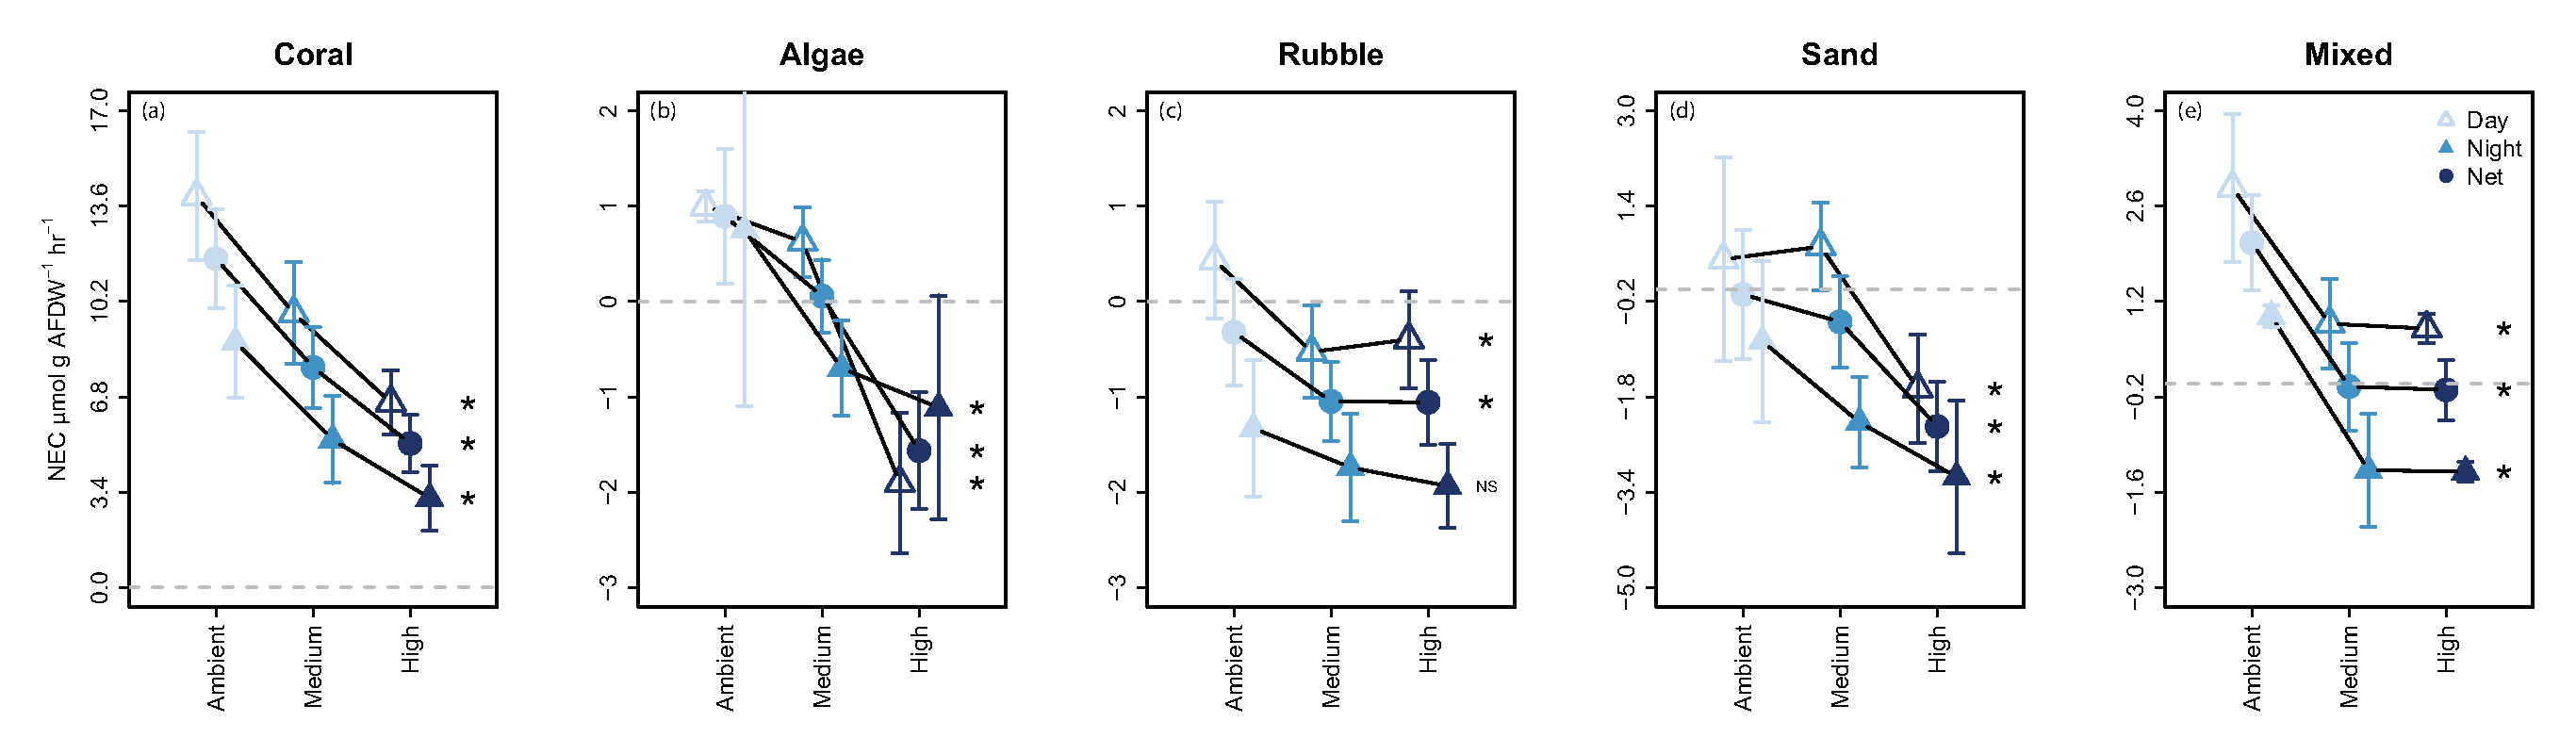
\includegraphics[width=6.5in]{MeanRates_NEC.eps}
%%% where xxxxxx name represents "figurename.eps"
\caption{NEC rates}
\label{NEC}
\end{figure}

\begin{figure}[!h]
\centering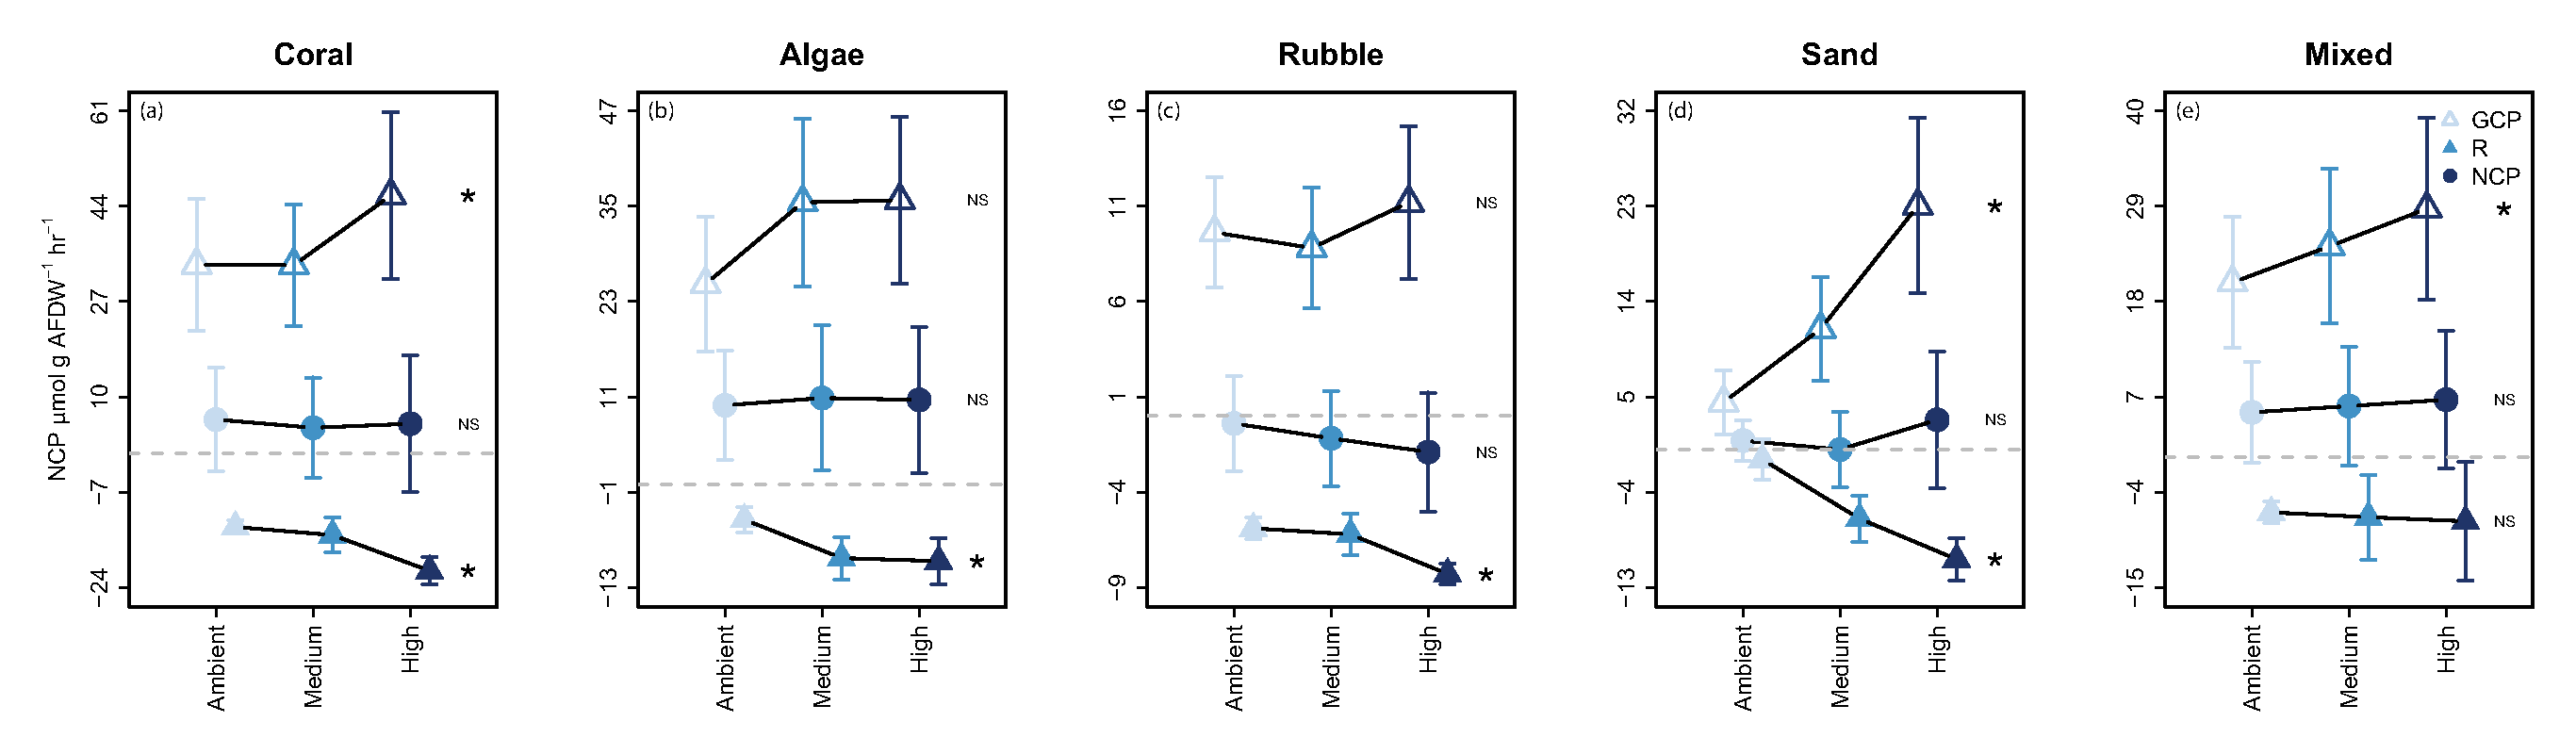
\includegraphics[width=6.5in]{MeanRates_NCP.eps}
%%% where xxxxxx name represents "figurename.eps"
\caption{NCP rates}
\label{NCP}
\end{figure}

\begin{figure}[!h]
\centering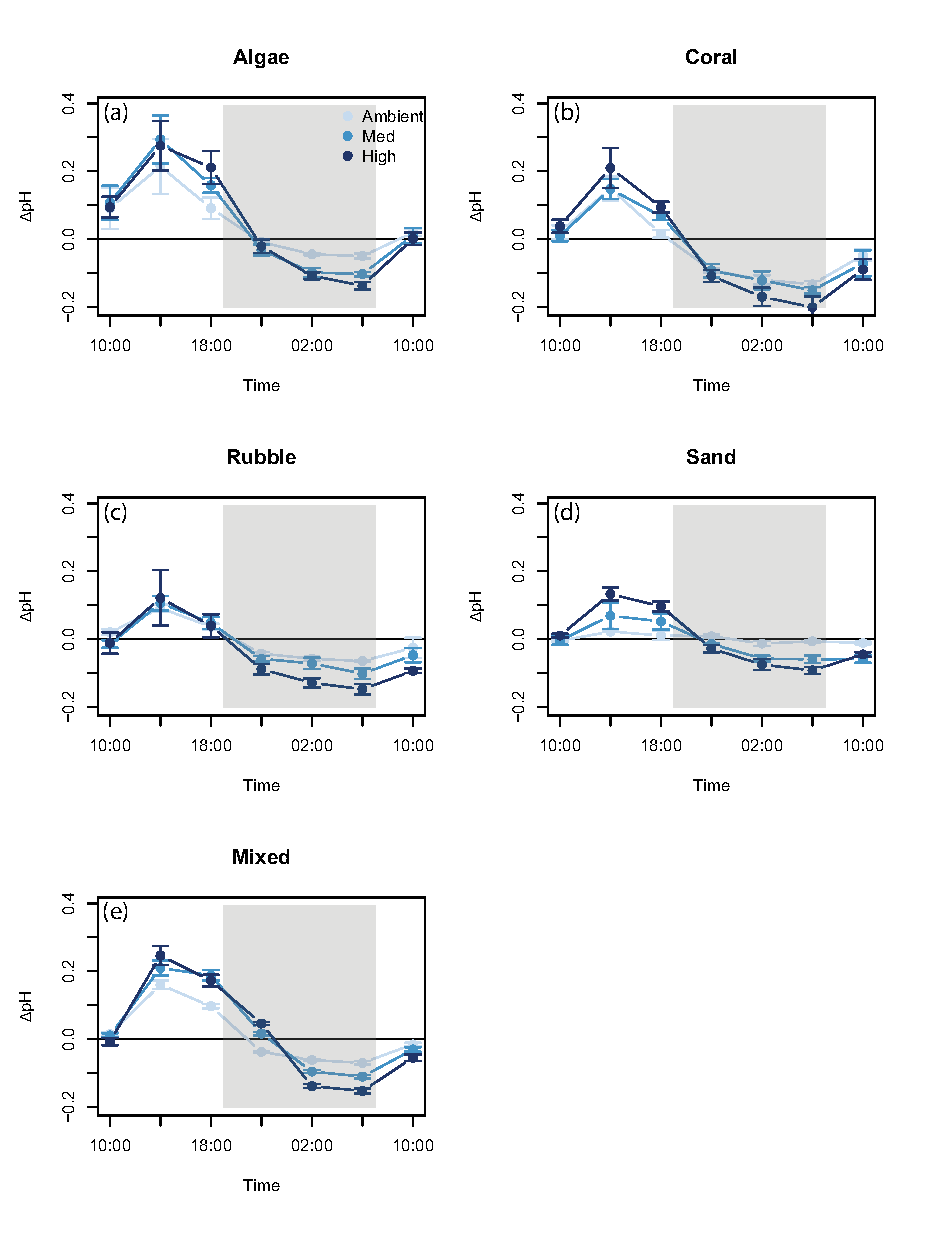
\includegraphics[width=6.5in]{DeltapHTime.eps}
%%% where xxxxxx name represents "figurename.eps"
\caption{Delta pH over time}
\label{DeltapH}
\end{figure}

\begin{figure}[!h]
\centering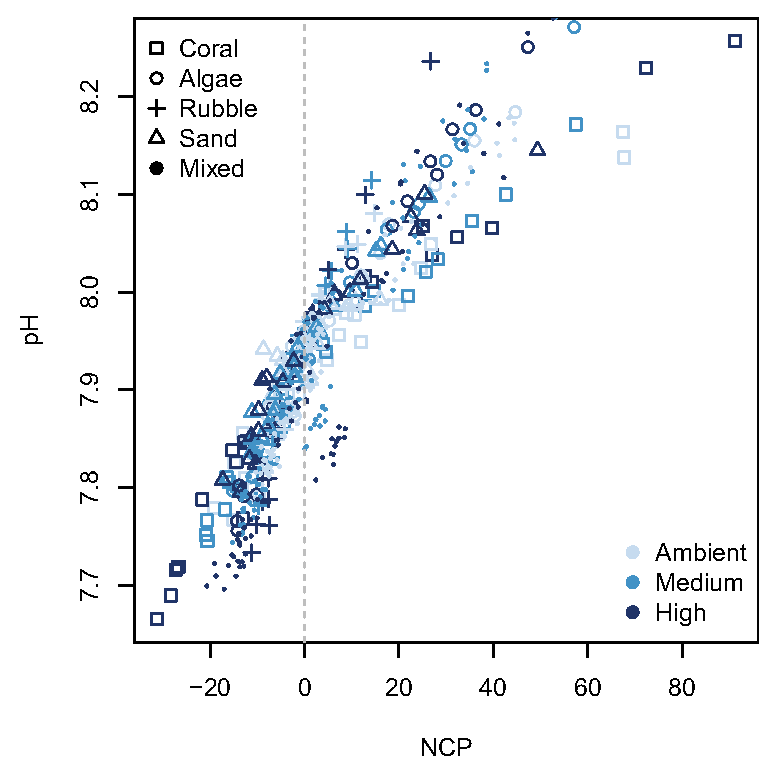
\includegraphics[width=6.5in]{NCPvspH.eps}
%%% where xxxxxx name represents "figurename.eps"
\caption{NCP vs pH}
\label{NCPvspH}
\end{figure}

\begin{figure}[!h]
\centering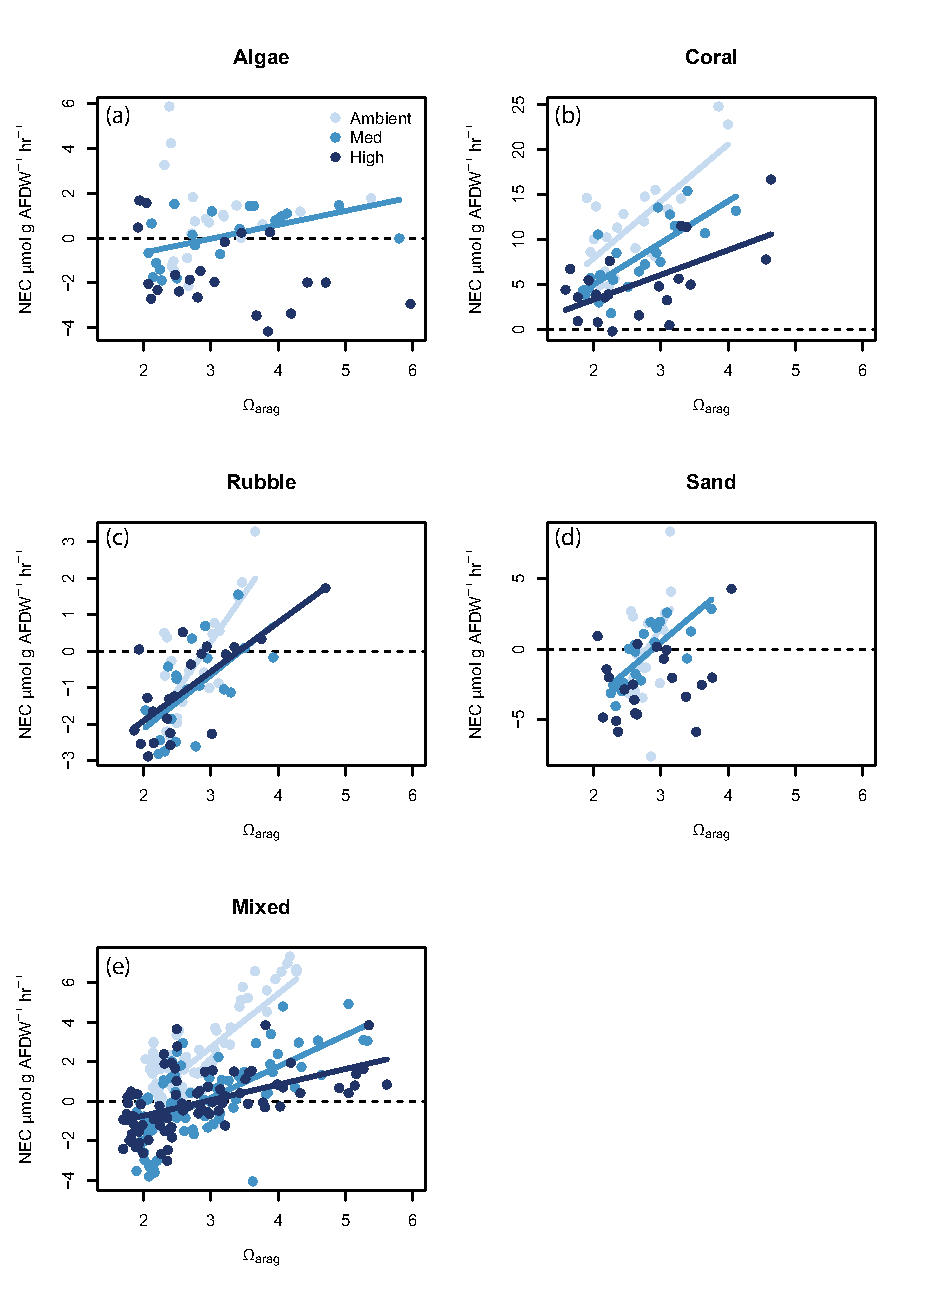
\includegraphics[scale=0.75]{NECvsOmega.eps}
%%% where xxxxxx name represents "figurename.eps"
\caption{NEC vs Omega}
\label{NECvsOmega}
\end{figure}

\vspace*{-10pt}



\begin{table}[!h]
\renewcommand{\thetable}{S\arabic{table}}
\caption{NEC Table}%%%Table caption goes here
\label{NECTable}
\end{table}%%%End of the table

\begin{table}[!h]
\renewcommand{\thetable}{S\arabic{table}}
\caption{NCP Table}%%%Table caption goes here
\label{NCPTable}
\end{table}%%%End of the table

\begin{table}[!h]
\renewcommand{\thetable}{S\arabic{table}}
\caption{pHvsNCP Table}%%%Table caption goes here
\label{pHvsNCPTable}
\end{table}%%%End of the table

\begin{table}[!h]
\renewcommand{\thetable}{S\arabic{table}}
\caption{Algae: NEC vs Omega}%%%Table caption goes here
\label{AlgaeOmegaTable}
\end{table}%%%End of the table

\begin{table}[!h]
\renewcommand{\thetable}{S\arabic{table}}
\caption{Coral: NEC vs Omega}%%%Table caption goes here
\label{CoralOmegaTable}
\end{table}%%%End of the table

\begin{table}[!h]
\renewcommand{\thetable}{S\arabic{table}}
\caption{Rubble: NEC vs Omega}%%%Table caption goes here
\label{RubbleOmegaTable}
\end{table}%%%End of the table

\begin{table}[!h]
\renewcommand{\thetable}{S\arabic{table}}
\caption{Sand: NEC vs Omega}%%%Table caption goes here
\label{SandOmegaTable}
\end{table}%%%End of the table

\begin{table}[!h]
\renewcommand{\thetable}{S\arabic{table}}
\caption{Mixed: NEC vs Omega}%%%Table caption goes here
\label{MixedOmegaTable}
\end{table}%%%End of the table


\section*{Acknowledgment}

Insert the Acknowledgment text here.


%%%%%%%%%% Insert bibliography here %%%%%%%%%%%%%%

%\begin{thebibliography}{9}
%\end{thebibliography}

\bibliography{Accretion_erosion.bib}
\bibliographystyle{prsb}
\end{document}